48. $\cfrac{7}{(x-1)(x-2)}+\cfrac{9}{x-2}+1\leqslant0\Leftrightarrow \cfrac{7+9x-9+x^2-2x-x+2}{(x-1)(x-2)}\leqslant0
\Leftrightarrow \cfrac{x(x+6)}{(x-1)(x-2)}\leqslant0.$ Применив метод интервалов, найдём ответ:
\begin{figure}[ht!]
\center{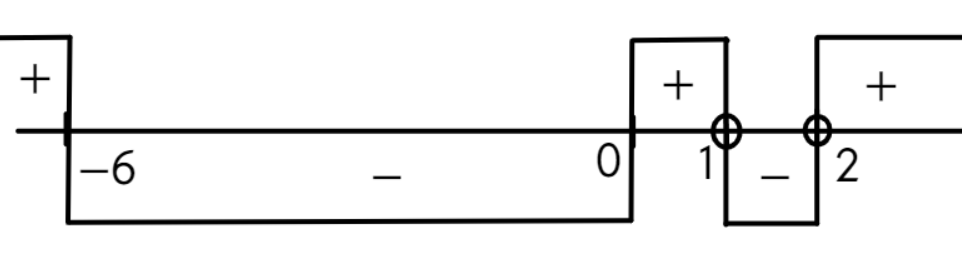
\includegraphics[scale=0.35]{int48.png}}
\end{figure}
$x\in[-6;0]\cup(1;2).$\newpage\noindent
